\documentclass{beamer}

%\usepackage{beamerthemesplit} // Activate for custom appearance
%\usepackage\{beamercolorthemedove}
%\setbeamertemplate{footline}[textline]{
%
\includegraphics[width=\paperwidth]{figures/datacron_logo.png}}
%}

\usepackage{textpos}
\usepackage{graphicx}
\usepackage{datetime}
\usepackage{tikz}
\usepackage[export]{adjustbox}
 %\usepackage{natbib}
 
 \usepackage{pgf}
 \usepackage{tikz}
 \usetikzlibrary{arrows,automata}
 %json%
\usepackage{minted}
%sudo apt-get install python-pygments
\usecolortheme{dove}

\def\datacronlogo{%
  \resizebox{!}{2.5ex}{
\includegraphics{figures/datacron_logo.png}%
}
}
\def\eclogo{
  \resizebox{!}{2.5ex}{
\includegraphics{figures/ec_logo.png}%
}
}
\def\horizonlogo{%
  \resizebox{!}{2.5ex}{
\includegraphics{figures/horizon_logo.png}%
}
}


\def\fraunhoferlogo{%
	\resizebox{!}{3.0ex}{
\includegraphics{figures/iais.pdf}%
	}
}
\def\unibonnlogo{%
	\resizebox{!}{3.0ex}{
\includegraphics{../chapters/figures/uni_bonn_logo_web.png}%
	}
}
%
\includegraphics[width=\paperwidth]{figures/datacron_logo.png}}

\title{	Distributed Online Learning for Large-scale Pattern Prediction over Real-time Event Streams}
%\author[shortname]{Author Name 1 \inst{1} \and Author Name 2 \inst{2}}
%\institute[shortinst]{\inst{1} affiliation for author1 \and %
 %                     \inst{2} affiliation for author2}
%\date{\today}

\defbeamertemplate*{footline}{example theme}
{%
    \begin{beamercolorbox}[wd=\paperwidth,ht=3.0ex,dp=1.125ex,%
        leftskip=.3cm,rightskip=.3cm plus1fil]{separation line}
        \usebeamerfont{section in head/foot}%
        \unibonnlogo\hfill\insertshorttitle\hfill\dmyydate \today\hfill \thepage \hfill \fraunhoferlogo
            \end{beamercolorbox}
}
\newcommand{\R}{\mathbb{R}}
\newcommand{\N}{\mathbb{N}}
\usepackage[numbers]{natbib}

\begin{document}

%\frame{\titlepage}

\frame{
	\begin{center}
		
		\textsc{\Large Rheinische\\[3mm] Friedrich-Wilhelms-Universität Bonn}\\[.8cm]
		
		\textsc{\Large Master Thesis Presentation}\\[1cm]

% Title
{ \Large \bfseries 
	%				Predicting patterns of moving objects based
	%				on contextual information with distributed online learning \\ 
	%				Distributed Online Learning for Forecasting Patterns of Moving Objects Events Streams \\
	Distributed Online Learning for Large-scale Pattern Prediction over Real-time Event Streams}\\[.8cm]

% Author and supervisor
\begin{minipage}[t]{0.4\textwidth}
	\begin{flushleft} \large
		%\emph{ }\\
		Ehab \textsc{Qadah}
	\end{flushleft}
\end{minipage}
\begin{minipage}[t]{0.5\textwidth}
	\begin{flushleft} \large
		\emph{First Examiner:} \\
		PD.~Dr.~Michael~\textsc{Mock} \\[0.3cm]
		\emph{Second Examiner:} \\
		
		Prof.~Dr.~Stefan \textsc{Wrobel} \\[0.5cm]
		
		%\emph{Abteilung:} \\
		%Autonome Intelligente Systeme
	\end{flushleft}
\end{minipage}

\vfill

% Bottom of the page
{\large  \hspace{1cm} \date{\dmyyyydate \today} }

\end{center}

}

	\begin{frame}<beamer>
		\frametitle{Outline}
		\tableofcontents
	\end{frame}


\section{Motivation and Problem Formulation}


%proof of concept 
%chalanges 
%requirments of stream processing %https://www.slideshare.net/arunkejariwal/modern-realtime-streaming-architec%tures?qid=f9d8532f-94be-47ee-bdf1-045826ba283e&v=&b=&from_search=1


\frame
{
	\frametitle{Motivation}
	\framesubtitle{A New Era: Big event Data streams}
		\begin{center}
		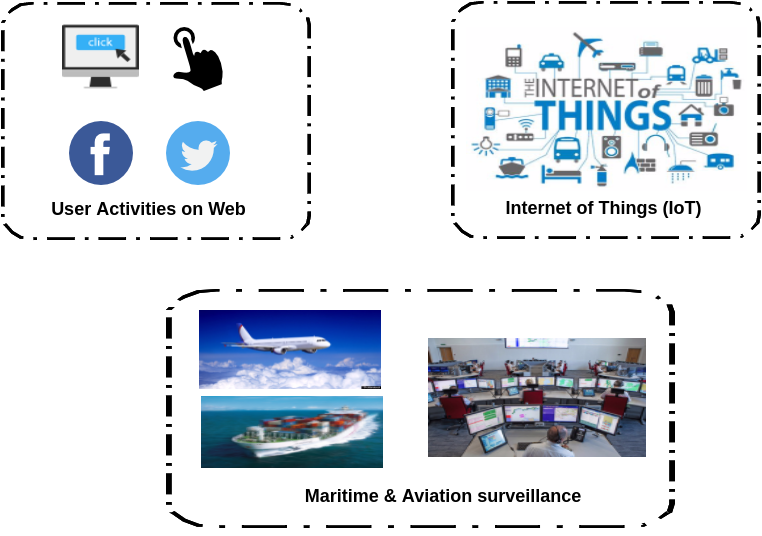
\includegraphics[scale=.36]{figures/motiv.png}\\
		.
	\end{center}
}


\frame
{
\frametitle{Motivation}
\framesubtitle{A New Era: Big event Data streams}
\begin{center}
	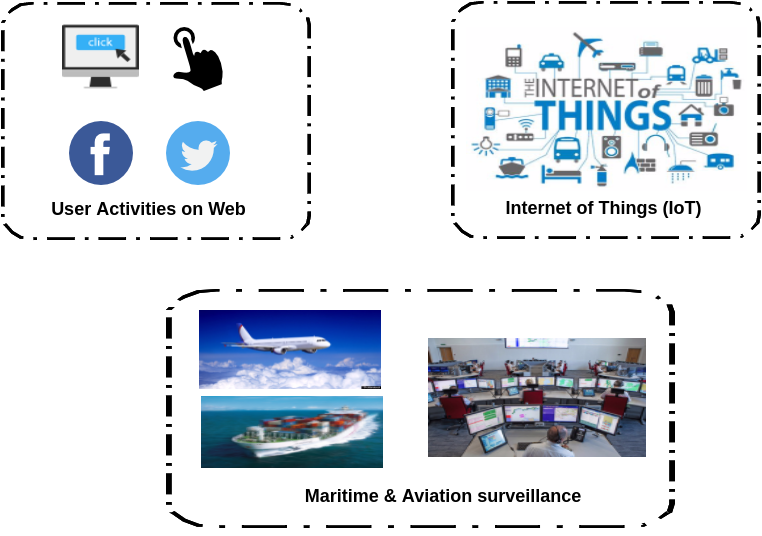
\includegraphics[scale=.27]{figures/motiv.png}\\
	.
\end{center}
	

	\begin{itemize}[]
		
		\item<1-> Common goal: recognition and prediction full matches of event patterns (situations of interest) in real-time.
%		\item<1-> improve operational efficiency.
%		\item<1 -> enable proactive decision making.
		
	\end{itemize}
}


\frame
{
	\frametitle{Problem Formulation}
	
	\begin{itemize}[]
		\item<only@1>Given a set of $k$ real-time streams of events $S = \{ s_1,s_2, ..., s_k\}$.
		
		\item<only@1> Each stream  $s_i=\langle e_1,e_3,...,e_t,...\rangle$  is a time-ordered infinite sequence of events.
		
		\item<only@1> Each event is defined as a tuple of attributes $e_i = (id,type,\tau,a_1,a_2,\ldots,a_n)$, where $type\ \in  \Sigma$ (i.e., event types), $\tau\in\R$, and  $id\in\N$ . 
		\item<only@1> A user-defined pattern $\mathcal{P}$ is given in the form of a regular expression over a set of event types. $\Sigma$ ($\mathcal{P} := E\ |\ \mathcal{P}_{1} ; \mathcal{P}_{2}\ | \mathcal{P}_{1} \vee \mathcal{P}_{2}\ |\ \mathcal{P}_{1}^{*}$,  $E \in \Sigma$).
		
		
		\item<2->The main objective is to predict the pattern $\mathcal{P}$ completion with certain probability in the future over each stream $s_i$ given the current time event $e_t$. 
		
		\item<3-> (\textbf{Pattern Prediction over Multiple Event Streams})
	\end{itemize}
}

%\begin{frame}[fragile]
%
%	\frametitle{An Illustrative Application Domain:}
%    \framesubtitle{Maritime Surveillance}
%	\begin{itemize}
%%		\item<only@1> Process  emitted from moving vessels or derived critical points of vessel trajectories as input event streams.
%		\item<only@1> Event tuple (i.e., critical points) derived from raw Automatic Identification System (AIS) messages of moving vessels e.g., 
%		\begin{minted}{json}
%	{
%	"timestamp":1443651492000,
%	"id":"228133000",
%	"annotation":"change_in_heading",
%	"latitude":48.117775,
%	"longitude":-4.4205885,
%	"distance":323.406,
%	"heading":264.27
%	"speed":18.48,
%	}
%	\end{minted}
%	
%		\item<only@1> Example patterns such as:\\
% 	   $\mathcal{P}_1=Sailing$ or\\ 
% 	   $\mathcal{P}_2=changeInHeading; gapStart; gapEnd; changeInHeading$
%	\end{itemize}
%\end{frame}


\section{The Proposed Approach}
\frame
{
	\frametitle{System Architecture \\ }
	%\framesubtitle{Maritime Surveillance}
	\begin{center}
	
		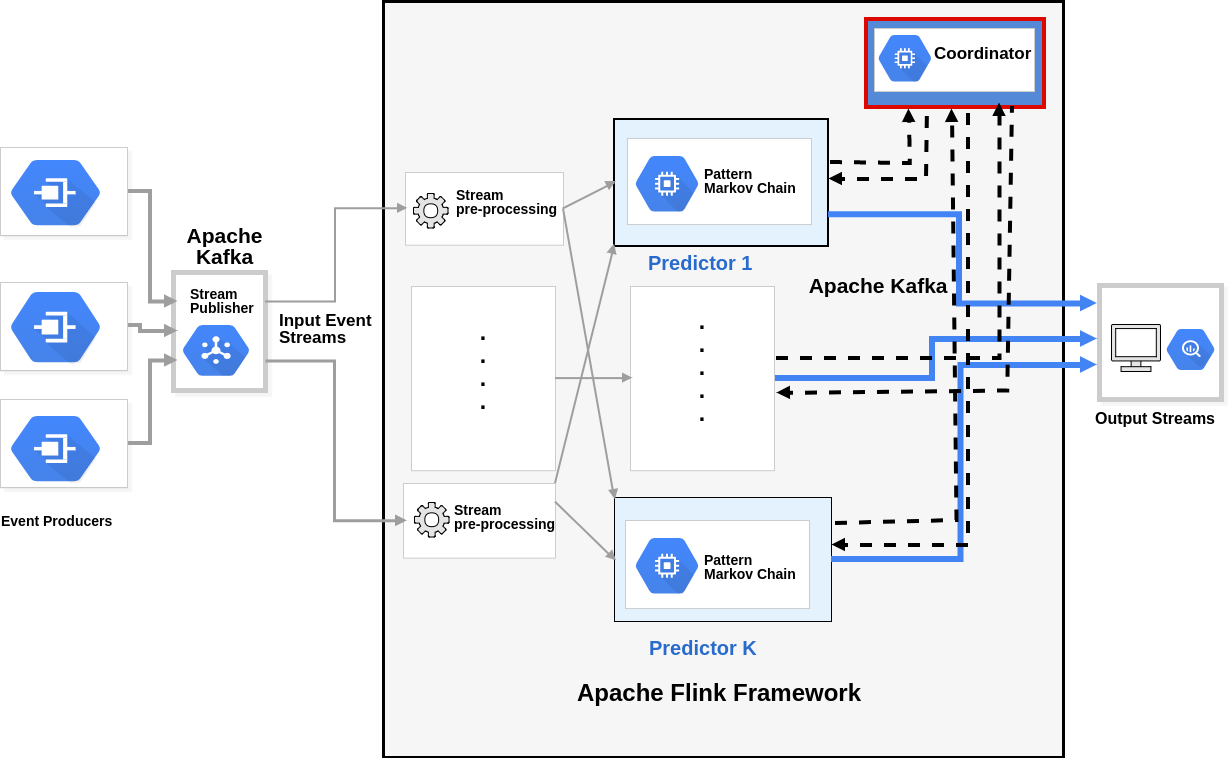
\includegraphics[width=\linewidth,left]{../chapters/figures/system.png}	\linebreak\\
	 .
		
%		emphasis on implementation // may add a slide // code link 
	\end{center}
}


\frame
{
	\frametitle{Scalable Pattern Prediction System \footnote{Source code: \url{https://goo.gl/BZ2Prk}.}}
	%\framesubtitle{Application Domain: Maritime Surveillance}
	\begin{itemize}
		
		\item<only@1> A scalable and distributed system that provides online pattern prediction over multiple real-time streams of events.
		\item<only@1> The proposed system is based on a novel method that combines  online probabilistic prediction models based on pattern Markov chain technique \cite{alevizos2017event} with a distributed online learning protocol \cite{kamp2014communication} to learn a global prediction model in a communication-efficient way.
		
	%	\item<only@1> The system maintains a Pattern Markov Chain prediction model for each event stream. 		
		\item<only@1> For large-scale processing support, the system is implemented on top of Apache Flink~\cite{carbone2015apache} along with Apache Kafka~\cite{Kafka}.
		
		%Apache Kafka is a scalable, fault-tolerant, and distributed streaming framework/messaging system \cite{Kafka}
		%on top of Apache Flink, a popular engine for distributed and large-scale stream processing. 
		\item<only@1> Developed in the context of the datAcron project \footnote{http://www.datacron-project.eu/}.
	\end{itemize}
}
\section{Event Forecasting with Pattern Markov Chains}
\frame
{
  \frametitle{ Event Forecasting with Pattern Markov
 	Chains \cite{alevizos2017event} }
	\framesubtitle{overview}
  \begin{itemize}[]
  	\item<1-> The model handles a single input stream $s_i$ of events.
  	\item<1-> The event stream $s_i$ is assumed to be generated by $m$-order Markov source.
  \item<1-> The  event pattern $\mathcal{P}$ is defined in the form of regular expressions over a finite set of event types $\Sigma$.

  \item<1-> A probabilistic model provides online forecasting reports when the $\mathcal{P}$ is expected to be completed in future. 
   
  \end{itemize}
}

\frame
{
	\frametitle{Event Forecasting with Pattern Markov
		Chains  }
	\framesubtitle{ How does it work?}
		\begin{itemize}
		\item<only@1> The pattern $\mathcal{P}=a ; d ; c$ is converted to deterministic finite automaton ($DFA$) with $\Sigma=\{a,b,c,d\}$. 
		
 \begin{figure}[ht]
	\begin{center}
		
	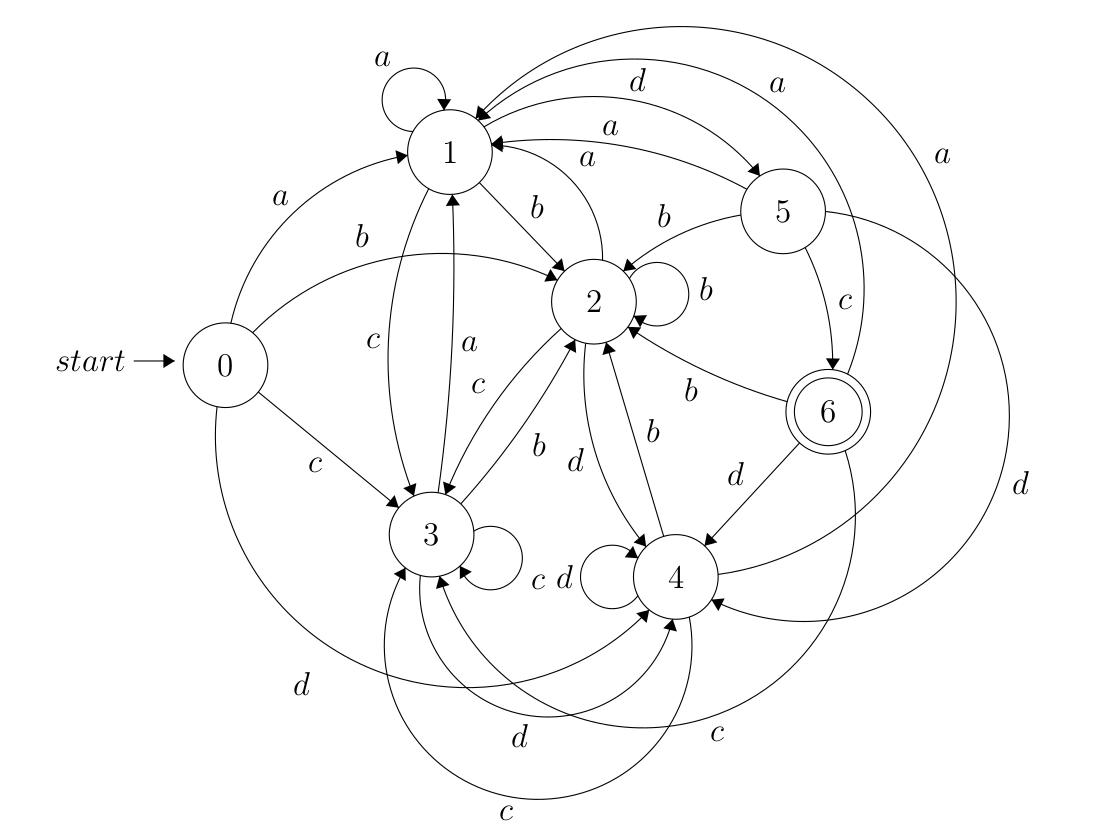
\includegraphics[width=\linewidth,height=.6\textheight,left]{figures/new/dfa.png}\linebreak
$Q=\{0,1,2,3,4,5,6\}$ for  $m=1$
\end{center}
%\caption[]{}
\end{figure}

	
			\end{itemize}
}

\frame
{
	\frametitle{Event Forecasting with Pattern Markov
		Chains}
	\framesubtitle{How does it work?}
	\begin{itemize}
		\item<only@1> The $DFA$ is used to construct a Markov chain, which is called a Pattern Markov Chain (\pmcmr).
		
		
	    \item<only@1> The states of $DFA$ is directly mapped to states of a transition probability matrix $\boldsymbol{\Pi}$  $\lvert Q \rvert \times \lvert Q \rvert$ of the \pmcmr.
		
		\item<only@1> 
	\begin{equation*}
	\label{eq:matrix_example}
	\boldsymbol{\Pi} = 
	\begin{Bmatrix} 
	0 \\ 1 \\ . \\ . \\6
	\end{Bmatrix}
	\begin{pmatrix} 
	p_{0,0}	    &. 		&. 		& . &  	p_{0,6} \\
    . 		    & .		& .	& .	& . \\
	.		    & .		& .		& .	& . \\
	.			& .		& .		& .	& .\\
	0			& .			& .		& .	&p_{6,6}
	\end{pmatrix}
	\end{equation*}
	
	\item<only@1> The maximum-likelihood estimator is used to compute the transition probabilities $p_{i,j}$ of the matrix $\boldsymbol{\Pi}$ 
	\begin{equation}
	\label{eq:pi_estim}
	\hat{p}_{i,j}=\frac{n_{i,j}}{\sum_{k \in Q} n_{i,k}}=\frac{n_{i,j}}{n_{i}}
	\end{equation}. 	
		
	\end{itemize}
}



\frame
{
	\frametitle{Event Forecasting with Pattern Markov
		Chains}
	\framesubtitle{Constructing the Pattern Prediction Model}
	\begin{itemize}
		
		\item<only@1> The probability distribution of the waiting-time (i.e., time required until the pattern is completed from state $q$) $P(W_{\mathcal{P}}(q)=n)$, is calculated based on the Markov chain transition matrix. 
	
		\begin{equation*}
		P(W_{\mathcal{P}}(q)=n)=\boldsymbol{\xi_{i}}^{T}\boldsymbol{N}^{n-1}(\boldsymbol{I}-\boldsymbol{N})\boldsymbol{1} 
		\end{equation*}
		where 
		\begin{equation}
		\label{eq:matrix}
		\boldsymbol{\Pi} = 
		\begin{pmatrix} 
		\boldsymbol{N} & \boldsymbol{C}  \\ 
		\boldsymbol{0} & \boldsymbol{I}
		\end{pmatrix}
		\end{equation}
		\item<only@1> The prediction intervals $I=(\mathit{start},\mathit{end})$ (i.e., the completion interval of the pattern $\mathcal{P}$ from the  current state $q$) are built using the waiting-time distribution $$P(I)=\sum_{n \in I}{W_{\mathcal{P}}(q)=n)} ,\ \textrm{and} \quad P(I) \geq  \theta_{p} \quad (end -start)\leq \theta_{s} $$. 
			
	\end{itemize}
}


\frame
{
	\frametitle{Event Forecasting with Pattern Markov
		Chains}
	\framesubtitle{Waiting-time distribution for
		$\mathcal{P}=a ; d ; c$, $\Sigma=\{a,b,c,d\}$, $m=1$.}
	\begin{figure}[]
		\begin{centering}
			\center
			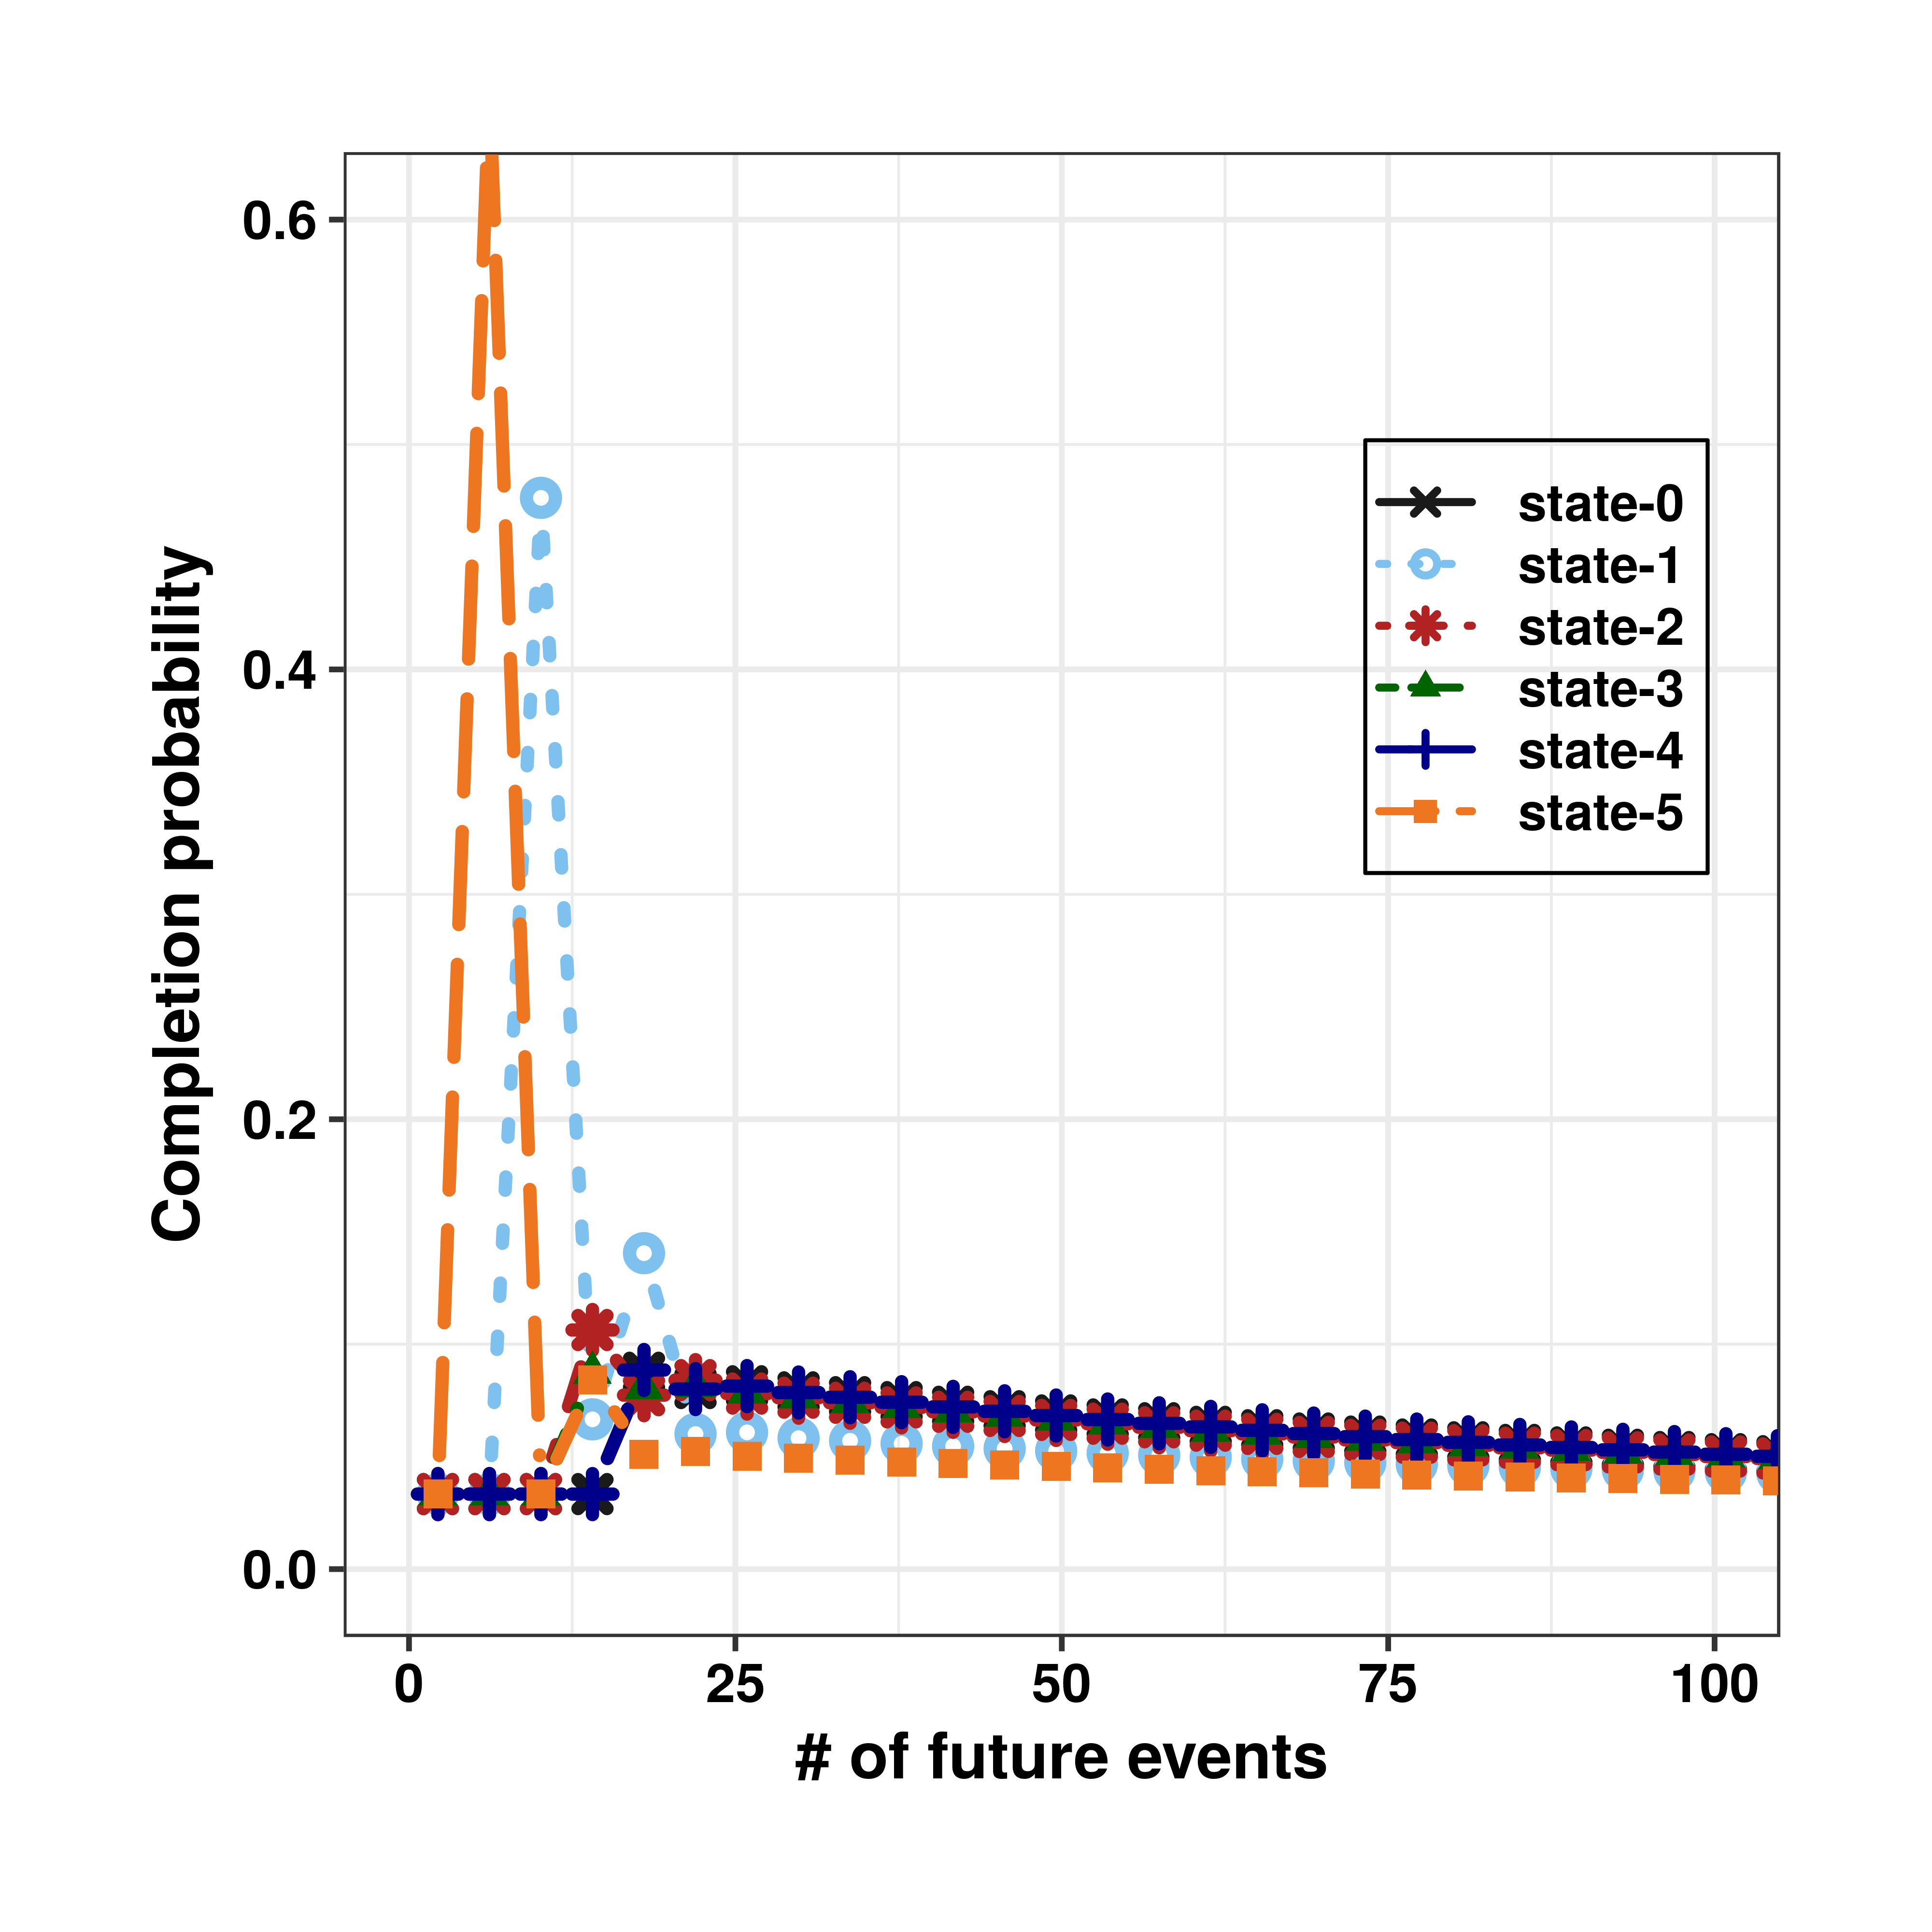
\includegraphics[width=.9\textwidth,height=.8\textheight]{../chapters/figures/new_wt.png}
			
			
			
		\end{centering}
	\end{figure}
	
	
}

\frame
{
	\frametitle{Event Forecasting with Pattern Markov
		Chains}
	\framesubtitle{Example of the computed prediction intervals for
		$\mathcal{P}=a ; d ; c$, $\Sigma=\{a,b,c,d\}$, $m=1$,$\theta_{p}=0.5,\ and\ \theta_{s}=20$.}
	
	\begin{figure}[]
		\begin{centering}
			\center
			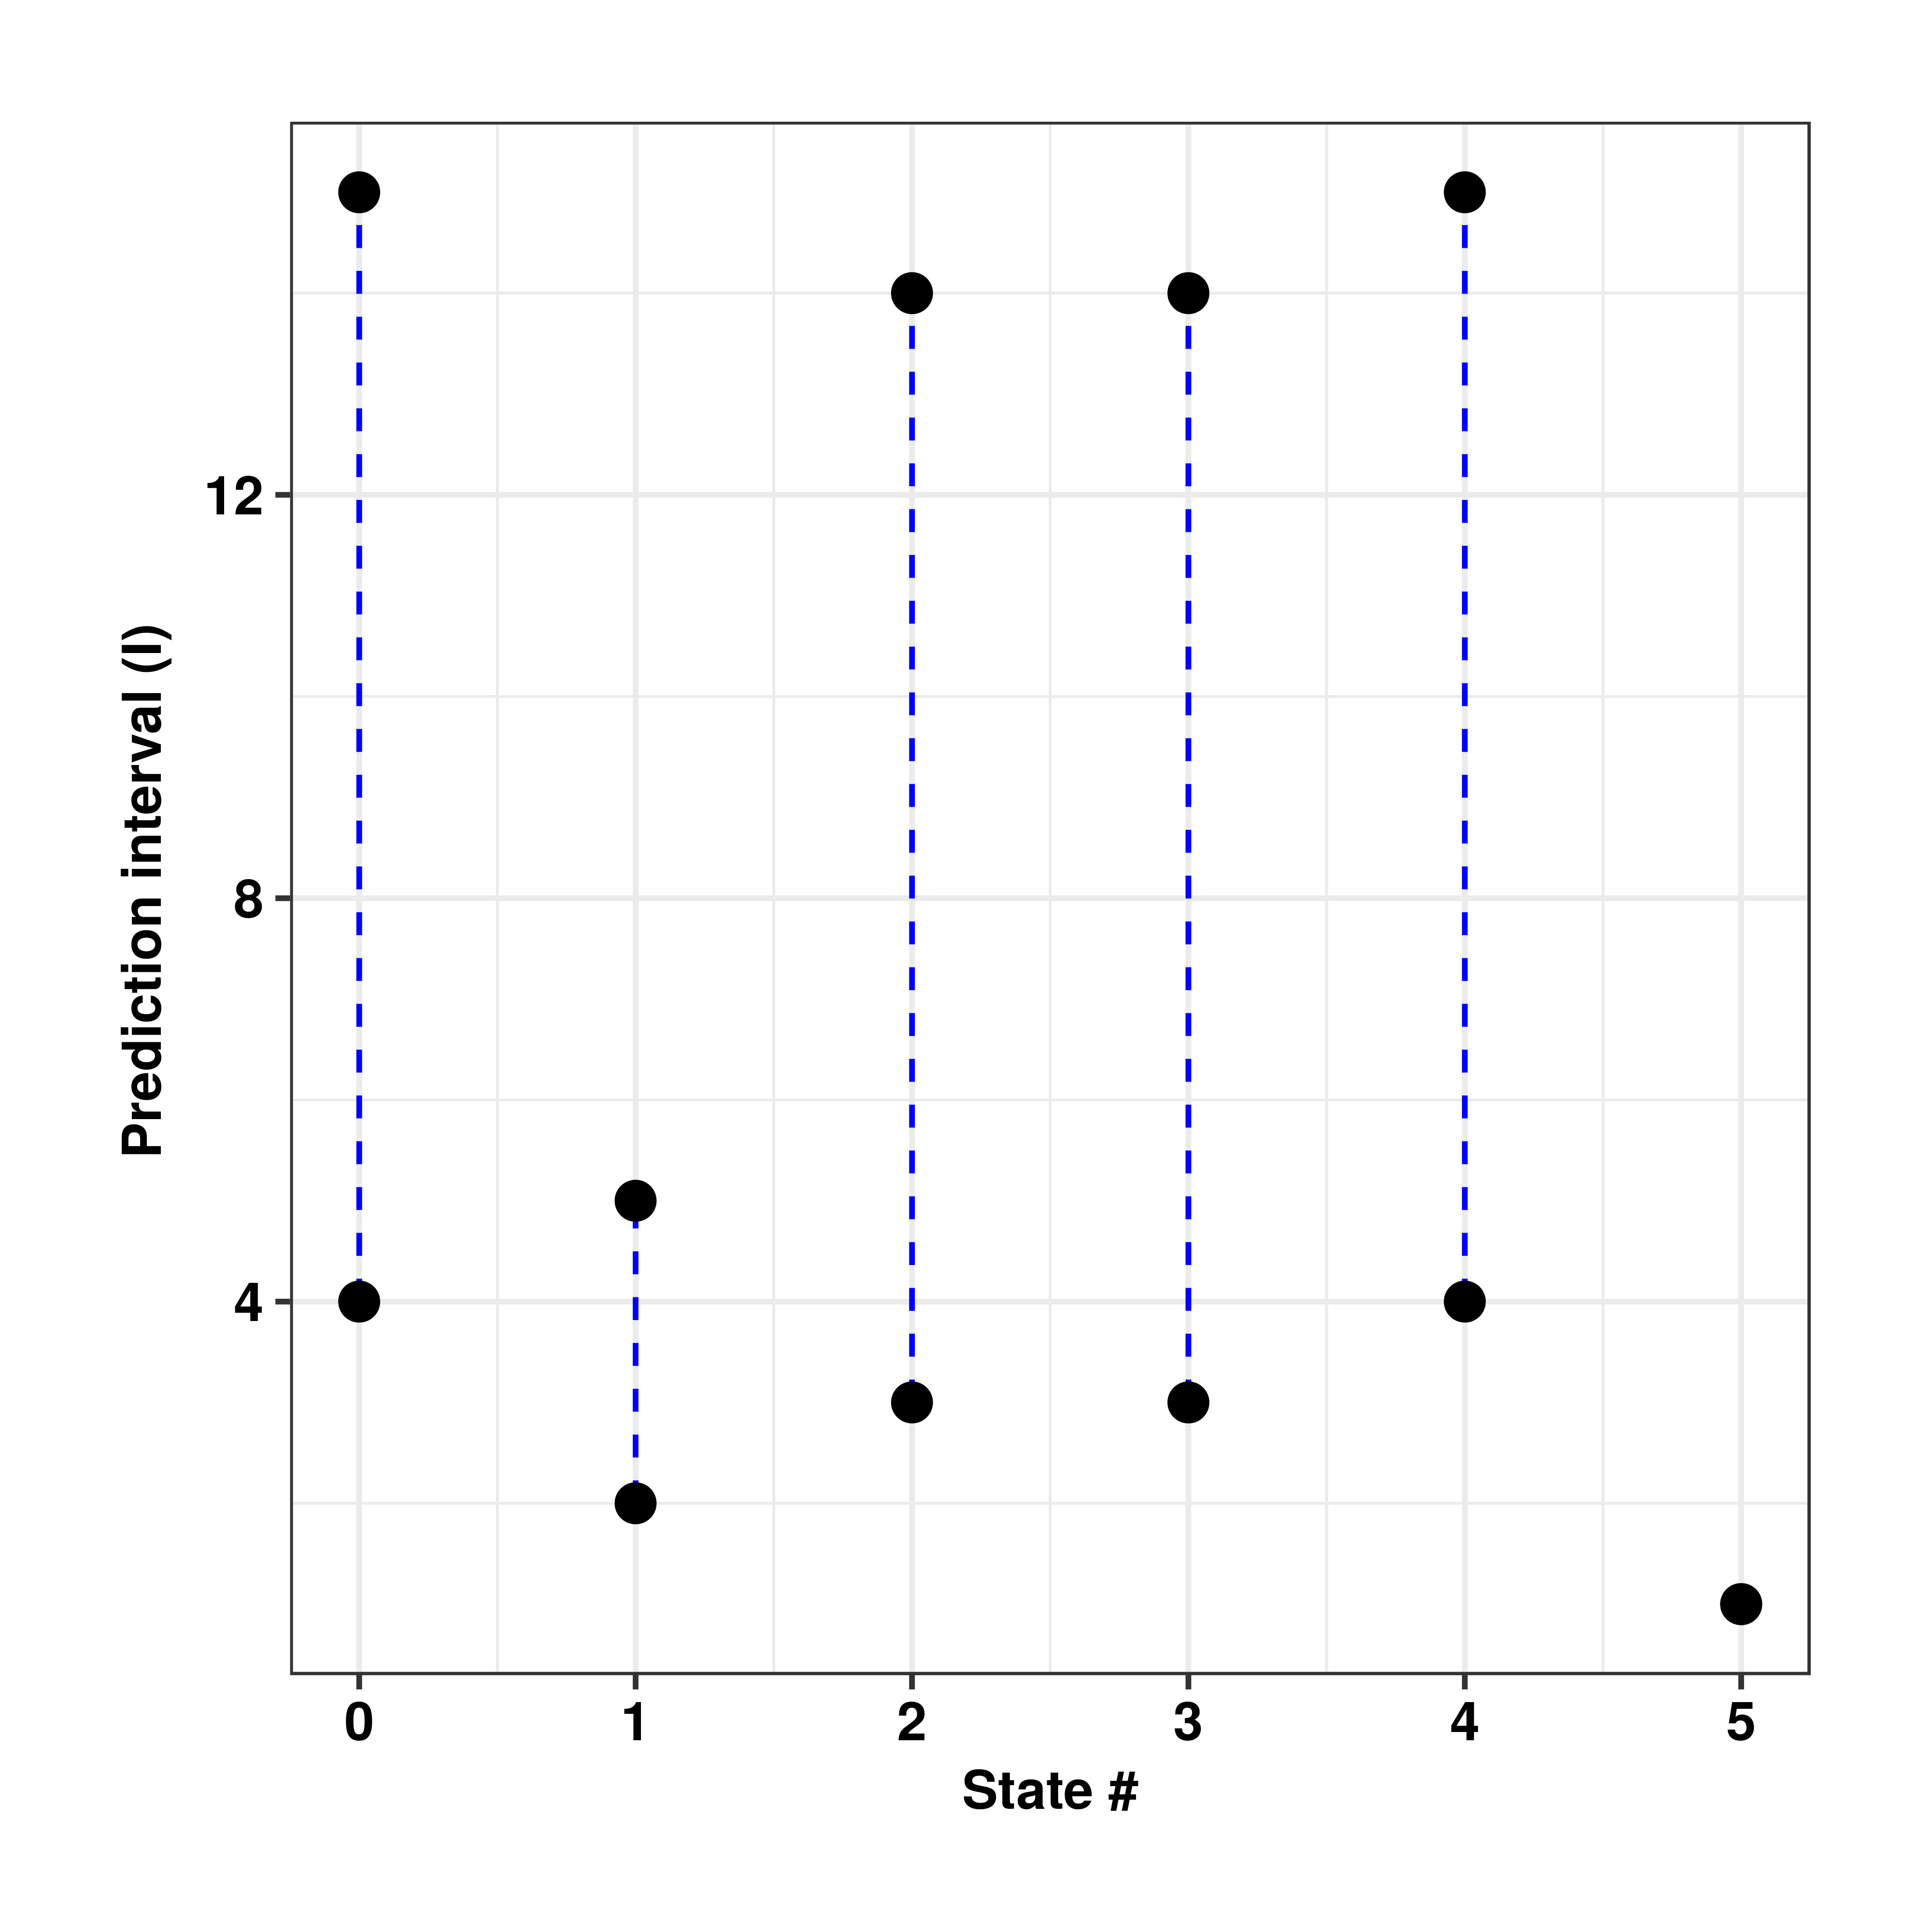
\includegraphics[width=.9\textwidth,height=.8\textheight]{../chapters/figures/new_prediction_intervals.png}
			
		\end{centering}
	\end{figure}
	
}


\frame
{
	\frametitle{Event Forecasting with Pattern Markov
		Chains}
	\framesubtitle{What is wrong?}
	\begin{itemize}
		
		\item<only@1> The overhead learning time of the Markov transition matrix for each input stream isolated from the others, how can we accelerate it?  
		 
		\item<only@1> The low performance of the model for an input event stream with less data. 
		
			\item<only@1> How can we enable the communication between the local models 
			 and leverage an aggregated global shared model in 
		 	a distributed and communication efficient fashion while maintaining
			provable and strong guarantees in service quality?
			
	
	\end{itemize}
}

\section{Distributed Online Learning for Pattern Prediction}
\frame
{
	\frametitle{Distributed Online Learning for Pattern Prediction}
	%\framesubtitle{Maritime Surveillance}
	%\framesubtitle{Proposed System Model}
	\begin{center}
		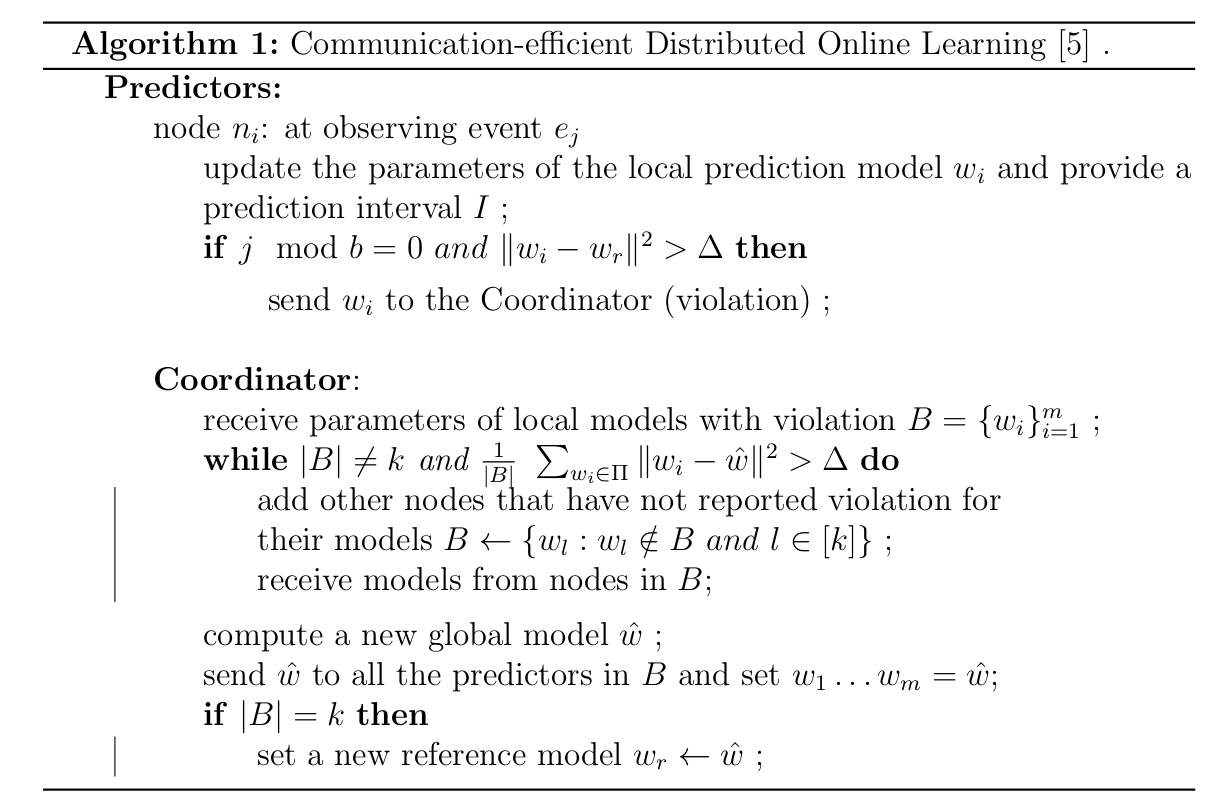
\includegraphics[width=\textwidth,left]{figures/new/dol.png}\\
.
	\end{center}
}


\frame
{
	\frametitle{ Communication-Efficient Distributed Online Prediction by Dynamic Model Synchronization  \citep{kamp2014communication}}
	\framesubtitle{}
	\begin{itemize}[]
		\item<1-> A protocol for distributed online prediction over multiple input data streams in a communication efficient manner.
		\item<1-> It allows to combine local models into a global model
	using a $synchronization$ $ operation$.
		\item<1-> The distributed learners exchange their local model with a central coordinator node periodically after observing a fixed number of data points (i.e., mini-batches) \citep{dekel2012optimal}.
		
		\item<1-> A dynamic synchronization scheme based on monitoring the local models variance from a global reference model ($\|f_i - r\|^2 \leq \bigtriangleup$).
		
		
%		dynamic synchronization scheme within which the learners communicate only if their local models diverge from a global reference point
	\end{itemize}
}

\frame
{
	\frametitle{Distributed Online Learning for Pattern Prediction}
		%\framesubtitle{Proposed Synchronization Operation}
	\begin{itemize}[]

	\item<1-> The
 $synchronization$ $ Operation$ for the global transition probability matrix $\hat{\Pi}$:
 \begin{equation*}
 \label{eq:dis_pi_estim}
 \hat{\pi}_{i,j} = \frac{\sum_{k \in K} n_{k,i,j}}{\sum_{k \in K} \sum_{l \in L} n_{k,i,l}}
 \end{equation*}

Where $n_{k,i,j}$ the number of transitions from state $i$ to state $j$ on node $k$.
	
\end{itemize}
}

\frame
{
	\frametitle{Distributed Online Learning for Pattern Prediction}
	%\framesubtitle{Proposed Synchronization Operation}
	\begin{itemize}[]
		
		\item<1->The divergence of the local models from the reference model $\|w_i - w_r\|^2$ is calculated by the sum of square difference between the local transition probability matrix $\Pi_i$ and the reference transition matrix $\Pi_r$:
		\begin{equation*}
		\label{eq:dis_pi_varinace}
		\|w_i - w_r\|^2=|\Pi_i - \Pi_r\|^2=\sum_{l,j} (\pi{i,l,j} -\pi{r,l,j})^2
		\end{equation*}
		
	\end{itemize}
}


\frame
{
	\frametitle{Distributed Online Learning for Pattern Prediction}
	\framesubtitle{Probabilistic Learning Guarantee}

		
		\begin{equation*}
		\begin{aligned}
		\label{eq:guarantee}
		\Pr\left( |\hat{\pi}_{i,j} - {p}_{i,j}| \geq c \right) \leq
		\frac{1}{k}\ \Pr\left( |\hat{p}_{i,j} - {p}_{i,j}| \geq c \right)
		\end{aligned}
		\end{equation*}
		
	
}
\section{Empirical Evaluation}
\chapter{Empirical Evaluation}

\label{chapter:evaluation}

\section{Evaluation Over Synthetic Event Streams}

\section{Evaluation Over Real-word Event Streams}
\label{sec:results}
In this section, we evaluate our proposed system by analyzing the predictive performance and communication complexity  using real-world event streams provided by the datAcron project in the context of maritime monitoring. The used event streams describe critical points (i.e., synopses) of moving vessels trajectories, which are derived from raw AIS messages as described in \cite{synopses1}. In particular, for our evaluation experiments we used a data set of synopses that contains $4,684,444$ critical points of $5055$ vessels sailing in the Atlantic Ocean during the period from 1 October 2015 to 31 March 2016.

\par We used the synopses data set to generate a simulated stream of event tuples  i.e., \textit{(id, timestamp, longitude, latitude, annotation, speed, heading)}, which are processed by the system to attach an extra attribute \textit{type} that represents the event value,  where $type$ $\in \Sigma$,  and $ \Sigma= \Sigma_1=$$\{$\textit{VerySlow, Slow, Moving,  Sailing, Stopping}$\}$ , which is based on a discretization of the speed values. Or $\Sigma=\Sigma_2=$ $\{$\textit{stopStart, stopEnd, changeInSpeedStart, changeInSpeedEnd,  slowMotionStart, slowMotionEnd, gapStart, gapEnd, changeInHeading}$\}$, which is derived based on the values of the $annotation$ attribute that encodes the extracted trajectory movement events \cite{synopses1}. In our experiments, we monitor a pattern $\mathcal{P}_1=Sailing$ with $\Sigma_1$ that detects when the vessel is underway (sailing). Likewise, we test a second pattern  $\mathcal{P}_2=$\textit{changeInHeading; gapStart; gapEnd; changeInHeading} with $\Sigma_2$.


\subsection*{Experimental setup} We ran our experiments on single-node standalone Flink cluster deployed on an Ubuntu Server 17.04 with Intel(R) Core(TM) i7-7700 CPU @ 3.60GHz X 8 processors and 32GB RAM. We used Apache Flink v1.3.2 and Apache Kafka v0.10.2.1 for our tests.


\subsection*{Evaluation criteria} Our goal is to evaluate our distributed pattern prediction system, which enables the synchronization of prediction models (i.e., PMC models) on the distributed predictor nodes. Our proposed system can operate in three different modes of  protocols/schemes of models synchronization: \begin{enumerate}[]
	\item static scheme based on synchronizing the prediction models periodically every $b$ of input events in each stream, 
\item continuous, full synchronization for each incoming event (hypothetical), 
\item dynamic synchronization protocol based on making the predictors communicate their local prediction models periodically but only under condition that the divergence of the local models from a reference model exceeds a variance threshold $\Delta$ (recommended).  	   

\end{enumerate}
\par We compare our proposed system against the isolated prediction mode, in which models are computed on single streams only, and compare the predictive performance in terms of :
\begin{enumerate}[]
	
\item  $\mathit{precision} =$ $ \mathit{\frac{\#\ of\ correct\ predictions}{\#\ of\ total\ predictions}}$ is the fraction of the produced predictions that are correct (i.e., a full match occurred within the prediction interval).   

\item $\mathit{spread} =end(I) -start(I)$ is the width of the prediction interval $I$. 

\end{enumerate} 
\par Moreover, we study the communication cost by measuring the $\mathit{cumulative\ communication}$ that captures the number of messages, which are required to perform the distributed online learning modes to synchronize the prediction models. Next, we present the experimental results for the patterns  $\mathcal{P}_1=Sailing$ with an order of $m=2$, and   $\mathcal{P}_2=$\textit{changeInHeading; gapStart; gapEnd; changeInHeading} with first order $m=1$. All experiments are performed with setting the batch size to 100  ($b=100$), the variance threshold of 2 ($\Delta=2$), $80\%$ as PMC prediction threshold ($\theta_{fc}=80\%$), and 200 for the maximum spread.

\begin{figure}[h]
	
	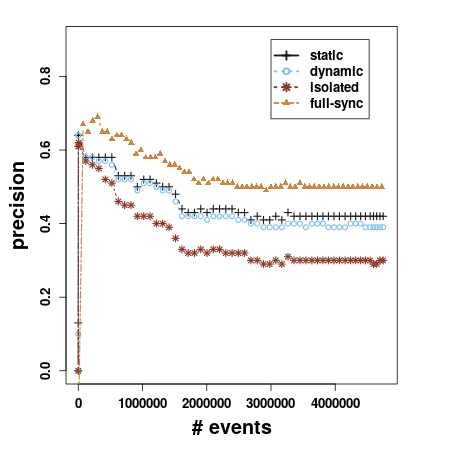
\includegraphics[width=\textwidth]{chapters/figures/precision_p1.png}
	
	\caption{Precision scores with respect to the number of input events over time for $\mathcal{P}_1$.}
	\label{fig:precsions}
\end{figure}

\subsection*{Experimental results} Figure ~\ref{fig:precsions} depicts the average precision scores of predictions models (one prediction model per vessel) of all synchronization modes for the first pattern $\mathcal{P}_1=Sailing$, namely, isolated without synchronization, continuous (full-sync), static, and our recommended approach based on the dynamic synchronization scheme. It can be clearly seen that all methods of distributed learning outperform the isolated prediction models. The hypothetical method of full continuous synchronization has the highest precision rates, while the static and dynamic synchronization schemes have close precision scores. Consequently, dynamic synchronization is not much weaker than the static synchronization, but requires much less communication, as explained below.
 

 
\par Figure ~\ref{fig:comm} provides the amount of the accumulated communication that is required by the three modes of the distributed online learning, while the isolated approach does not require any communication between the predictors. These results are shown  for $\mathcal{P}_1$.  As expected, a larger amount of communication is required for the continuous synchronization comparing to the static and dynamic approaches. Also, it can be seen that we can reduce the communication overhead by applying the dynamic synchronization protocol (a reduction by a factor of 100) comparing to the static synchronization scheme, even with a small variance threshold $\Delta=2$. Furthermore,  the dynamic  protocol is still preserving a close predictive performance to the static one (see Figure ~\ref{fig:precsions}).  Therefore, we will only consider the dynamic synchronization and the isolated approach in the  evaluation of the second pattern.

\begin{center}
	
	\begin{figure}[]
		
		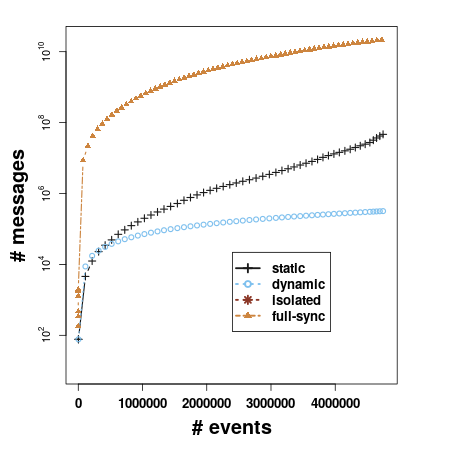
\includegraphics[width=\textwidth]{chapters/figures/messages_p1.png}
		
		\caption{Commutative communication with respect to the number of input events over time for $\mathcal{P}_1$.}
		\label{fig:comm}
	\end{figure}
\end{center}




\begin{center}
	
	\begin{figure}[]
		
		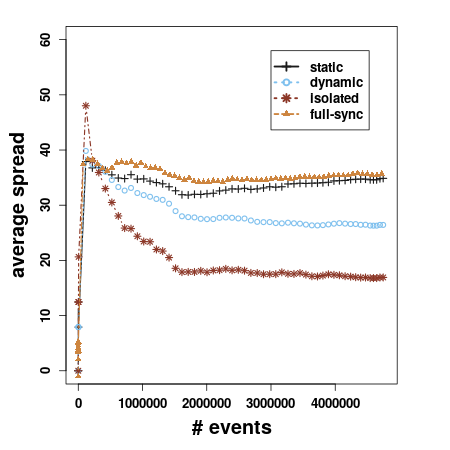
\includegraphics[width=\textwidth]{chapters/figures/spread_p1.png}
		
		\caption{Average spread value for $\mathcal{P}_1$.}
		\label{fig:spread}
	\end{figure}
\end{center}

 \begin{figure}[]
	
	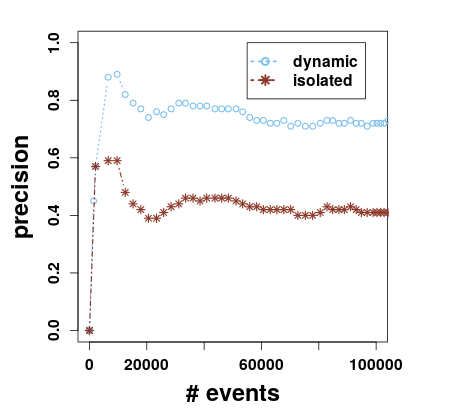
\includegraphics[width=\textwidth]{chapters/figures/precision_p2.png}
	
	\caption{Precision scores of $\mathcal{P}_2$  for \textit{PLEASURE CRAFT} vessels.}
	\label{fig:precsions_p2}
\end{figure}

\par In Figure ~\ref{fig:precsions}, we also noted that the precision is going down in a first phase and stabilizes then.  This seems to be counter-intuitive, as the models should improve when getting more data up to a certain point. For explanation, we have investigated the effect of the distributed synchronization of the prediction models on the average spread value, Figure  ~\ref{fig:spread}  shows the spread results for all approaches. It can be seen that the spread is higher for the distributed learning based methods comparing to the isolated approach. Furthermore, the average spread is decreasing over time until convergence, as result of confidence increase in the models. This may explain the drop in the precision scores from the beginning until reaching the convergence. We will investigate further in the interrelation between precision and spread in future work. 


\par For the second, more complex pattern ($\mathcal{P}_2$), we have found that the precision was worse for a distributed model generated over all vessels than in the model created for each vessel in isolation. This indicates that there is no  global model describing the behavior of all models consistently. However, when looking at specific groups of vessels, we achieved an improvement in terms of precision. As initial experiment, we only enable the synchronization of the prediction models associated with vessels that belong to the same vessel class. Currently, this change is technically performed by an extra filter step that passes only one type of vessels, while multiple runs of the system are required for all vessel types. For example, Figure ~\ref{fig:precsions_p2} shows the precision scores for vessels of class \textit{PLEASURE CRAFT}. An interesting observation is that the dynamic synchronization approach still has  a higher precision scores than the isolated approach. We will further investigate the effect of groupings and more patterns in future work.







%\par In Table ~\ref{tab:recall}, we present the mean of the recall scores for the both patterns in the all approaches It can be seen that the different approaches have a close recall scores, while the most frequent pattern ($\mathcal{P}_1$) has a lower recall than $\mathcal{P}_2$.
%
%\begin{table}[h]
%	\caption{Average recall for  $\mathcal{P}_1$ and $\mathcal{P}_2$.}
%	\label{tab:recall}
%	\begin{tabular}{lcc}
%		\toprule
%		Approach &Mean recall for $\mathcal{P}_1$ &Mean recall for $\mathcal{P}_2$\\
%		\midrule
%		isolated & 0.1707  &0.947 \\
%		static & 0.1754  &  0.960 \\
%		dynamic & 0.174  & 0.0.964 \\
%		full-sync & 0.1817  & 0.972 \\
%		\bottomrule
%	\end{tabular}
%\end{table}


 

\section{Future Work and Conclusion}

\chapter{Conclusion and Future Work}
\label{chap:conclusions}

In this chapter, we discuss the results of our system, and some of the aspects of underlying method. Also we give some proposals for future work.




\section{Conclusion}
%In this paper, we have presented a system that provides  a distributed pattern prediction over multiple large-scale event streams of moving objects (vessels). The system uses the event forecasting with Pattern Markov Chain (PMC) \cite{alevizos2017event} as the base prediction model on each event stream, and it applies the protocol for distributed online prediction \cite{kamp2014communication} to exchange information between the prediction models over multiple input event streams.  Our proposed system has been implemented using Apache Flink and Apache Kafka, and empirically tested against large real-world event streams related to trajectories of moving vessels. As future work, we will investigate the effect of grouping the input event streams on the predictive performance of our proposed system. Furthermore,  we will study the interrelation between precision and spread scores.



\section{Future Work}
%\begin{itemize}[noitemsep]
%	\item In some practical applications the input event streams may belong to different distributions, we propose to divide the input event streams into similar groups, in order to combine the corresponding predictions models to construct a representative global model in each group. The aggregation operation refers to the synchronization operation (e.g., joint average of the local models) in the distributed online learning protocol, which is performed by a central coordinator that constructs and distributes a global prediction model for the input event streams based on the  local models.
%	\item temporal patterns 
%	\item another communication media  
%	\item theoretical analysis of dynamic protocol 
%	\item another transition probabilities learning technique 
%	\item another weighted sync operator
%	
%	
%	%	 it seems that predicted patterns currently concern individual objects (hence each one is monitored by a distinct predictor), although in reality there may be interactions and correlations among moving objects. As a future research direction, perhaps it would be worth briefly discussing whether and how this method could be extended to handle such correlated events involving multiple objects (e.g., a group of vessels heading to a place).
%	
%	
%\end{itemize}

%\section{}
\frame
{
  \frametitle{Work  Plan }
	
 
  	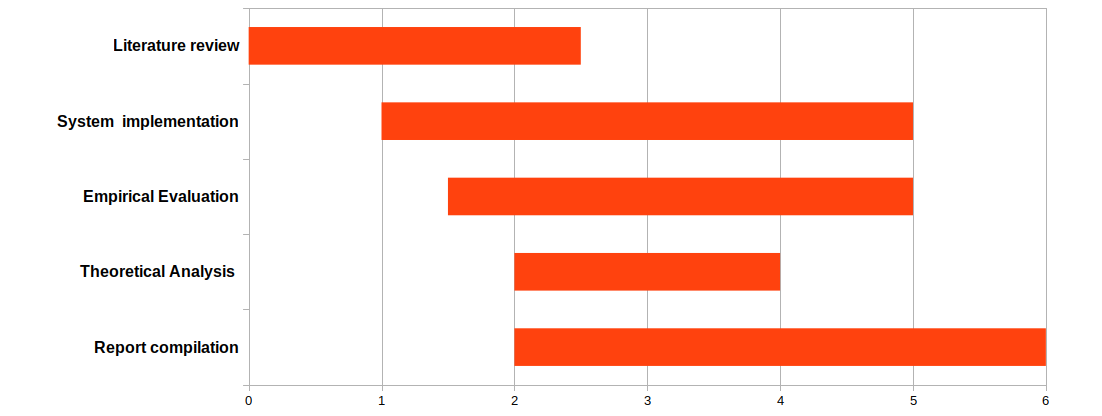
\includegraphics[width=1.1\textwidth,left]{figures/plan.png}\\
  	
  
}

%\begin{frame}
%\frametitle{Tasks}
%\begin{columns}
%\begin{column}{0.5\textwidth}
%  \begin{itemize}
%  \item<1->Task 1. 
%  \end{itemize}
%\end{column}
%\begin{column}{0.5\textwidth}  %%<--- here
%  \begin{itemize}
%  \item<1-> Task 2. 
%  \end{itemize}
%\end{column}
%\end{columns}
%\end{frame}

\begin{frame}[allowframebreaks]
	\frametitle{Bibliography}
	\bibliographystyle{plainnat} 
	\bibliography{myrefs2}
	
\end{frame}


\begin{frame}
	
	%\frametitle{Synchronization Schemes }
	%\framesubtitle{Evaluation Metrics}
	\centering
	
	\textsc{\Large Questions?}\\[1.5cm]
	
	Thank you!
\end{frame}
\end{document}
